

% Chapter 1

\chapter{Introducción} % Main chapter title

\label{Chapter1} % For referencing the chapter elsewhere, use \ref{Chapter1} 

\lhead{Capítulo 1. \emph{Introducción}} % This is for the header on each page - perhaps a shortened title

%----------------------------------------------------------------------------------------

%--------------------------------------------------------
%Sección 1
%--------------------------------------------------------


\begin{figure}[htbp]
	\centering
		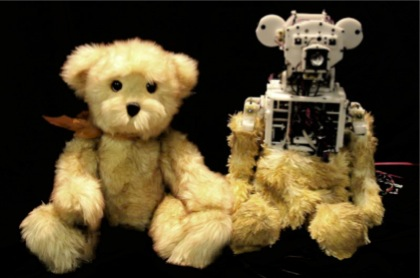
\includegraphics[width=0.8\textwidth]{./Figures/robot.jpg}
		\rule{35em}{0.5pt}
	\caption[Robot Huggable]{Robot creado por MIT Media Lab para cuidados personales. Imagen tomada de \cite{Stiehl:2006:HTR:1179133.1179149}}
	\label{fig:Huggable}
\end{figure}

En la década de 1990, teniendo tan solo 6 años me encontraba escondido en la logia de la casa de mis padres, que estaba ubicada en pleno barrio Ñuñoa Santiago, desarmando cuanto artefacto cayera en mis manos. Según recuerdo, más lo que mi madre me cuenta, desarmé el único teléfono que había en la casa. Era uno de esos que ya no se ven, que hacen uso un dial con pulsos para marcar el número. Tal era mi curiosidad sobre esta máquina, que la desarme completamente solo para tratar de entender como se producía ese sonido sin igual que llamaba la atención de toda persona que estuviera en la casa. Por su puesto mi madre me retó porque no pude volver a armarlo, pero en secreto siempre supe que ella y mi padre se divertían con mis pequeñas aventuras. En esta misma casa, mi padre intento montar una empresa de consultores con unos amigos, lo que significaba que al lado de mi pequeño taller clandestino tenía a mi disposición 3 o 4 computadores con sus flamantes pantallas Hércules donde pasé tardes completas jugando los primeros vídeo juegos y sin darme cuenta mis primeros pasos en la computación. Algo más grande, cuando tenía 13 años, por el trabajo de mi padre nos fuimos a vivir a Concepción. Una ciudad bien particular, ya que el invierno da mucho tiempo para estar en el hogar. Ahí tuve mi primer gran acercamiento a la computación, recuerdo que mientras mis compañeros estaban en clases de ingles en la sala, yo me escabullía para ir directo a las salas de computación, donde el encargado me permitía ayudarle a instalar Windows 95 en los computadores. Disquete tras disquete íbamos intercambiándolos en cada computador hasta lograr que el famoso logo de la ventana saliera en la pantalla. Desde esa época que familiares y amigos me han pedido ayuda con sus maquinas. En la enseñanza media volvimos como familia a Santiago, volví a mi colegio de infancia, el Liceo San Agustín, donde junto a dos compañeros nos inscribimos en mi primer concurso, el concurso escolar de robótica de la UDP. Aquí alumnos de la universidad nos enseñaron como se podía construir y programar un robot, no fue fácil y luego de un par de meses entre tantos manuales y la simbología alienígena (diagramas eléctricos) tomamos la decisión de retirarnos. En el año 2005 ingresé a la UTFSM, llegué el 2006 a Valparaíso y lo primero que vi en el patio central fue un pequeño cartel que decía: "Taller del Centro de Robótica", junto a otro amigo que hice apenas ingresé a la USM entusiasmados con esta idea de hacer nuestros propios robots, no lo dudamos y nos inscribimos para ser parte de este grupo de alumnos. Una vez dentro del Centro de Robótica (CR), conocí mucha gente con intereses similares a los míos, con gran conocimiento y más que nada, una gran solidaridad para compartir este conocimiento. Tardes completas dedicadas a aprender las oscuras artes de la electrónica, luchando con la frustración de armar un circuito y que este no funcionara a la primera, fui paso a paso avanzando hasta poder construir mis primeros robots. Argo fue el primer proyecto de robótica en que me incluí, este se trataba de construir un robot cuadrúpedo capaz de moverse en todas las direcciones en un plano utilizando la menor cantidad posible de grados de libertad. Luego vino LALO, proyecto que se destacó por ser de los primeros robots en hacer uso de un Smartphone como cámara y controlador motores. En la actualidad me interesa más poder transmitir los conocimientos que tengo para introducir a la gente en las nuevas tecnologías que existen que están al alcance de todos.

Hacer Robots en Valparaíso no es una tarea sencilla, la falta de lugares especializados para comprar dificulta contar con los componentes necesarios para construir una máquina.

Al comienzo de este proyecto se trabajó en Santiago de Chile, en conjunto con la Universidad de Chile (UChile) bajo la tutela del Doctor Juan Cristóbal Zagal en el Laboratorio de Síntesis de Máquinas Inteligentes. Por parte de la Universidad Técnica Federico Santa María (USM), se trabajó con la Doctora María José Escobar, del Departamento de Electrónica y luego se incorporó el Doctor Pablo Prieto del Departamento de Diseño de Productos. El financiamiento para realizar este prototipo ha sido por parte de las dos Instituciones, Universidad Técnica Federico Santa María y Universidad de Chile.

Durante el proceso de desarrollo se tuvieron que hacer diversas compras de materiales, pero los lugares más recurrentes al momento de hacerlas fueron Olimex y Casa Royal. La primera es una empresa dedicada a traer productos para hacer prototipos y construir máquinas, la segunda cuenta con varios insumos básicos para trabajar en desarrollo de circuitos electrónicos. Ambas empresas se encuentran en Santiago, por lo que trabajar en esta ciudad es de gran ayuda para reducir los tiempos en desarrollo.
Luego de armar un primer robot funcional, con materiales disponibles en Santiago de Chile, se hizo una búsqueda en internet de componentes en tiendas especializadas.

Este trabajo resume el desarrollo del proyecto MODI, que es un robot simple de construir que tiene como fin ser repetible para facilitar la construcción de Enjambres de robots. Primero hay una breve explicación de que es un robot, luego las herramientas necesarias para construir un robot como MODI, después se detalla el robot y junto con su construcción, y al final algunas aplicaciones.



%----------------------------------------------------------------------------------------

% Antes de comenzar con el trabajo aproyecho de escribir que ha sido mucha la gente que me ha ayudado en el camino y espero este trabajo pueda inspirar a cualquiera que se interesen por la robótica y la tecnología.
